\documentclass[12pt,a4paper]{article}
\usepackage[utf8]{inputenc}
\usepackage[english]{babel}
\usepackage{amsmath}
\usepackage{amsfonts}
\usepackage{amssymb}
\usepackage{graphicx}
\usepackage[left=2cm,right=2cm,top=2cm,bottom=2cm]{geometry}
\begin{document}

\raggedright

\section*{Questionnaire}

\begin{enumerate}
\item Do you need these for deep learning?
\begin{itemize}
	\item Lots of math T / \textbf{F}
	\item Lots of data T / \textbf{F}
	\item Lots of expensive computers T / \textbf{F}
	\item A PhD T / \textbf{F}
\end{itemize}

\item Name five areas where deep learning is now the best in the world. \\

\begin{enumerate}
	\item natural language processing
	\item computer vision
	\item medicine and biology
	\item image generation
	\item recommendation systems
\end{enumerate}

\item What was the name of the first device that was based on the principle of the artificial neuron? \\

\smallbreak

Mark I Perceptron

\bigbreak

\item Based on the book of the same name, what are the requirements for parallel distributed processing (PDP)? \\

\begin{itemize}
	\item[1.] a set of \textit{processsing units}
	\item[2.] a \textit{state of activation}
	\item[3.] an \textit{output function} for each unit
	\item[4.] a \textit{pattern of connectivity} among units
	\item[5.] a \textit{propagation rule} for propagating patterns of activities through the network of connectivities
	\item[6.] an \textit{activation rule} for combining the inputs impinging on a unit with the current state of that unit to produce an output for the unit
	\item[7.] a \textit{learning rule} whereby patterns of connectivity are modified by experience
	\item[8.] an \textit{environment} within which the system must operate
\end{itemize}

\item What were the two theoretical misunderstandings that held back the field of neural networks? \\

\smallbreak

Marvin Minsky and Seymour Papert wrote a book called \textit{Perceptrons}, where they showed a single layer of neural nodes were unable to learn some simple but critical mathematical functions (such as XOR). In theory, adding just one extra layer of neurons was enough to allow any mathematical function to be approximated with these neural networks, but in practice (back then) such networks were often too big and too slow to be useful.

\bigbreak

\item What is a GPU? \\

\smallbreak

A graphics processing unit (GPU) is a special kind of processor that can perform multiple (thousands) of tasks at a time, especially designed for displaying 3D environments in video games.

\bigbreak

\item Open a notebook and execute a cell containing: 1+1. What happens? \\

\smallbreak

In a Jupyter Notebook, executing 1+1 will output 2.

\bigbreak

\item Why is it hard to use a traditional computer program to recognize images in a photo? \\

\smallbreak

The computer doesn't know what to look for to recognize what objects are in an image. In general, for a computer program, we give it a list of instructions based roughly on how a human would do so, but it is hard to write down instructions for a computer to recognize objects since we ourselves aren't sure of the process; our brain automatically recognizes things.

\bigbreak

\item What did Samuel mean by "weight assignment"? \\

\smallbreak

Weights are just variables, and a weight assignment is a particular choice of values for those variables.

\bigbreak

\item What term do we normally use in deep learning for what Samuel called "weights"? \\

\smallbreak

Parameters.

\bigbreak

\item Draw a picture that summarizes Samuel's view of a machine learning model. \\

\smallbreak

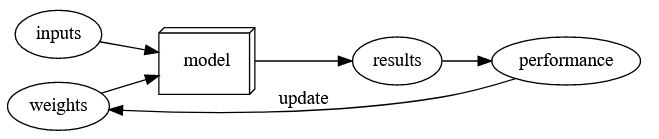
\includegraphics[scale=1]{model.jpeg}

\bigbreak

\item Why is it hard to understand why a deep learning model makes a particular prediction? \\

\smallbreak

Think of a deep learning model as a human brain in a way. There are many processes that go into us formulating a thought or classifying an animal as a cat or a dog. Deep neural networks have thousands of layers of neurons. It is hard to determine what factors went into determining the final output and how important each factor was. Each layer of the network interact with each other, with each layer feeding to other layers. Because of the complex nature of deep learning models, it is very difficult why a neural network outputs a given prediction.

\bigbreak

\item What is the name of the theorem that shows that a neural network can solve any mathematical problem to any level of accuracy? \\

\smallbreak

The \textbf{universal approximation theorem} states that neural networks can theoretically represent any mathematical function. However, because of the limitations of available data and computer hardware, it is practically impossible to do so.

\newpage

\item What do you need in order to train a model? \\

\item How could a feedback loop impact the rollout of a predictive policing model? \\

\item Do we always have to use 224×224-pixel images with the cat recognition model? \\

\item What is the difference between classification and regression? \\

\item What is a validation set? What is a test set? Why do we need them? \\

\item What will fastai do if you don't provide a validation set? \\

\item Can we always use a random sample for a validation set? Why or why not? \\

\item What is overfitting? Provide an example. \\

\item What is a metric? How does it differ from "loss"? \\

\item How can pretrained models help? \\

\item What is the "head" of a model? \\

\item What kinds of features do the early layers of a CNN find? How about the later layers? \\

\item Are image models only useful for photos? \\

\item What is an "architecture"? \\

\item What is segmentation? \\

\item What is y\_range used for? When do we need it? \\

\item What are "hyperparameters"? \\

\item What's the best way to avoid failures when using AI in an organization?

\end{enumerate}

\section*{Further Research}

\begin{enumerate}

\item Why is a GPU useful for deep learning? How is a CPU different, and why is it less effective for deep learning? \\

\item Try to think of three areas where feedback loops might impact the use of machine learning. See if you can find documented examples of that happening in practice.
\end{enumerate}






\end{document}